\documentclass[11pt,a4paper,notitlepage,fleqn,final]{article}

\usepackage{amsmath}
\usepackage{amsfonts}
\usepackage{amssymb}
\usepackage{libs/commath2}
\usepackage{xcolor}
\usepackage[hidelinks]{hyperref}
\usepackage[skins,theorems]{tcolorbox}
\usepackage{titlesec}
\usepackage{circuitikz}
\usepackage{pgfplots}
\usepackage{mathtools}
\usepackage[makeroom]{cancel}
\usepackage{mathrsfs}
\usepackage{wrapfig}
\usepackage{subcaption}
\usepackage{floatrow}
\usepackage{esint}
\usepackage{enumitem}
\usepackage{bm}
\usepackage{relsize}
\usepackage{xfrac}
\usepackage{comment}
\usepackage{siunitx}
\usepackage{MnSymbol}
\usepackage[obeyDraft]{todonotes}

\pgfplotsset{compat=1.14}
\usetikzlibrary{arrows.meta}
\usetikzlibrary{patterns}
\usetikzlibrary{decorations.pathmorphing,patterns}
\usetikzlibrary{decorations.markings}
\usetikzlibrary{backgrounds}
\usetikzlibrary{shapes.misc}
\usetikzlibrary{shapes.multipart}
\usetikzlibrary{snakes}
\usetikzlibrary{fadings}
\usetikzlibrary{intersections}
\usetikzlibrary{arrows.meta}
\usetikzlibrary{calc}
\usetikzlibrary{matrix}

\tikzset{cross/.style={cross out, draw,
        minimum size=2*(#1-\pgflinewidth),
        inner sep=0pt, outer sep=0pt}}
\tikzset{
    mark position/.style args={#1(#2)}{
        postaction={
            decorate,
            decoration={
            	post length=1mm, % ??? Magic to fix "Dimension
            	pre length=1mm, % ???  too large" errors.
                markings,
                mark=at position #1 with \coordinate (#2);
            }
        }
    }
}

\pgfmathdeclarefunction{sinc}{1}{%
	\pgfmathparse{abs(#1)<0.01 ? int(1) : int(0)}%
	\ifnum\pgfmathresult>0 \pgfmathparse{1}\else\pgfmathparse{sin(#1 r)/#1}\fi%
}

\usepackage[left=2cm,right=2cm,top=2cm,bottom=2cm]{geometry}

%\usepackage[no-math]{fontspec}
\usepackage{fontspec}
%\usepackage{mathspec}
\usepackage{unicode-math}
\setmainfont{texgyretermes-regular.otf}
\setsansfont{texgyreheros-regular.otf}
%\newfontfamily\greekfont[Script=Greek]{Linux Libertine O}
%\newfontfamily\greekfontsf[Script=Greek]{Linux Libertine O}
\usepackage{polyglossia}
\newfontfamily\greekfont[Script=Greek]{texgyretermes-regular.otf}
\newfontfamily\greekfontsf[Script=Greek]{texgyreheros-regular.otf}
\newfontfamily\greekfonttt[Script=Greek]{Latin Modern Mono}
%\usepackage[greek]{babel}
\setdefaultlanguage{greek}
\setotherlanguage{english}
\newcommand{\textlatin}[1]{#1}
%\newcommand{\mathlarger}{}

%\usepackage[utf8]{inputenc}
%\usepackage[greek]{babel}


%\usepackage{tkz-euclide} % loads  TikZ and tkz-base
%\usetkzobj{angles} % important you want to use angles

\newlist{enumparen}{enumerate}{1}
\setlist[enumparen]{label=(\arabic*)}
\newlist{enumpar}{enumerate}{1}
\setlist[enumpar]{label=\arabic*)}

\newlist{enumgreek}{enumerate}{1}
\setlist[enumgreek]{label=\alph*.}
\newlist{enumgreekparen}{enumerate}{1}
\setlist[enumgreekparen]{label=(\alph*)}
\newlist{enumgreekpar}{enumerate}{1}
\setlist[enumgreekpar]{label=\alph*)}


\newlist{enumroman}{enumerate}{1}
\setlist[enumroman]{label=(\roman*)}

\newlist{enumlatin}{enumerate}{1}
\setlist[enumlatin]{label=(\alph*)}

\newlist{invitemize}{itemize}{1}
\setlist[invitemize]{noitemsep,label=}

\input{libs/fiximplies}

\makeatletter
\let\anw@true\anw@false

%\newcommand{\attnboxed}[1]{\textcolor{red}{\fbox{\normalcolor\m@th$\displaystyle#1$}}}
\makeatother
\tcbset{highlight math style={enhanced,colframe=red,colback=white,%
        arc=0pt,boxrule=1pt,shrink tight,boxsep=1.5mm,extrude by=0.5mm}}
\newcommand{\attnboxed}[1]{\tcbhighmath[colback=red!5!white,drop fuzzy shadow,arc=0mm]{#1}}
\titleformat{\section}{\bf\Large}{Κεφάλαιο \thesection}{1em}{}
\newtcolorbox{attnbox}[1]{colback=red!5!white,%
    colframe=red!75!black,fonttitle=\bfseries,title=#1}
\newtcolorbox{infobox}[1]{colback=blue!5!white,%
    colframe=blue!75!black,fonttitle=\bfseries,title=#1}

\AtBeginDocument{%
\let\arg\relax
\let\Re\relax
\let\Im\relax
\DeclareMathOperator{\arg}{Arg}
\DeclareMathOperator{\Re}{Re}
\DeclareMathOperator{\Im}{Im}
}
\DeclareMathOperator{\sinc}{sinc}
\DeclareMathOperator{\Res}{Res}

\newif\ifhidetikz
\hidetikzfalse
%\hidetikztrue   % <---- comment/uncomment that line

\ifhidetikz

\let\oldtikzpicture\tikzpicture
\let\oldendtikzpicture\endtikzpicture

\renewenvironment{tikzpicture}{
    \tiny
    \tt
    \color{blue}
    \newcommand{\draw}{\textit{draw}}
    \newcommand{\filldraw}{\textit{filldraw}}
    %\newcommand{\x}{\textit{x}}
    %\newcommand{\p}{\textit{x}}
    \newcommand{\x1}{\textit{x1}}
    \newcommand{\y1}{\textit{y1}}
    \newcommand{\p1}{\textit{p1}}
}{
}
\newenvironment{axis}{
    \newcommand{\addplot}{\textit{addplot}}
}{
}
\fi

\newtcbtheorem[number within=section]{theorem}{Θεώρημα}%
{colback=green!5,colframe=green!35!black,colbacktitle=green!35!black,fonttitle=\bfseries,enhanced,attach boxed title to top left={yshift=-2mm,xshift=-7mm},width=.9\textwidth,arc=.7mm}{th}
\newtcbtheorem[number within=section]{defn}{Ορισμός}%
{colback=blue!5,colframe=cyan!35!black,colbacktitle=blue!35!black,fonttitle=\bfseries,enhanced,attach boxed title to top left={yshift=-2mm,xshift=-2mm}}{def}
\newtcbtheorem[number within=section]{exercise}{Άσκηση}%
{colback=gray!3,colframe=gray!35!black,colbacktitle=gray!35!black,fonttitle=\bfseries,enhanced,attach boxed title to top left={yshift=-2mm,xshift=-2mm}}{exc}




\title{Θεωρία Σημάτων και Γραμμικών Συστημάτων
	\\
	{
	\normalsize Σημειώσεις από τις παραδόσεις
	}}
\date{2016
	\\
	{
	\small Τελευταία ενημέρωση: \today
	}
	}
\author{
	Για τον κώδικα σε \LaTeX, ενημερώσεις και προτάσεις:
\\
 \url{https://github.com/kongr45gpen/ece-notes}}

\setmainfont{Linux Libertine O}
\setsansfont{Ubuntu}
%\newfontfamily\greekfont[Script=Greek]{Linux Libertine O}
%\newfontfamily\greekfontsf[Script=Greek]{Linux Libertine O}
\usepackage{polyglossia}
\newfontfamily\greekfont[Script=Greek,Scale=0.95]{GFS Artemisia}


\begin{document}
	\maketitle

	\tableofcontents

	\include{signals/chap0}
    \include{signals/chap1}
	\include{signals/chap2}
	\include{signals/chap3}


    \section{Θεώρημα Δειγματοληψίας}
    \begin{gather*}
    	X(f) = \int_{-\infty}^{\infty} x(t) e^{-j2\pi ft}\dif t\\
    	x(t) = \int_{-\infty}^{\infty} X(f) e^{j2\pi f t}\dif t\\
    	x_1(t) x_2(t) \xrightarrow{\mathscr F} X_1(f)*X_2(f)\\
    	X_1(f) X_2(f) \xrightarrow{\mathscr F^{-1}} x_1(t)*x_2(t)\\
    	\mathrm{sinc} (t) = \frac{\sin(\pi t)}{\pi t}
    \end{gather*}

    Συνάρτηση δειγματοληψίας: \(
    \displaystyle S_{T_s}(t) = \sum_{n=-\infty}^\infty
    \delta(t-nT_s) \xrightarrow{\mathscr F} F_p \sum_{n=-\infty}^\infty
    \delta(f-nF_p) \qquad F_p=\frac{1}{T_s}
     \)

    \begin{tikzpicture}
    	\draw[->] (-3,0) -- (3,0);
    	\draw (0,0) -- (0,3);

    	\draw[thick,blue,->] (-2,0) -- (-2,1.5);
    	\draw[thick,blue,->] (-1,0) -- (-1,1.5);
    	\draw[thick,blue,->] (0,0) -- (0,1.5);
    	\draw[thick,blue,->] (1,0) -- (1,1.5);
    	\draw[thick,blue,->] (2,0) -- (2,1.5);

    	\draw[<->] (1,-0.2) --(2,-0.2) node[below,midway] {$T_s$};

    	\draw (4,1.5) node {\(
    		\xrightarrow{\qquad
    			\mathlarger{\mathlarger{\mathlarger{\mathscr F}}}\qquad
    			}
    		\)};

 	    \draw (6,0) -- (11,0);
 	    \draw[->] (8.4,0) -- (8.4,3);

 	    \draw[thick,blue,->] (6.8,0) -- (6.8,1.5);
 	    \draw[thick,blue,->] (7.6,0) -- (7.6,1.5);
 	    \draw[thick,blue,->] (8.4,0) -- (8.4,1.5);
 	    \draw[thick,blue,->] (9.2,0) -- (9.2,1.5);
 	    \draw[thick,blue,->] (10,0) -- (10,1.5);

 	    \draw[<->] (9.2,-0.2) --(10,-0.2) node[below,midway] {$F_p = \frac{1}{T_s}$};
    \end{tikzpicture}

    \begin{gather*}
    	S_{F_s}(f) \xrightarrow{\mathscr F^{-1}} T_p S_{T_p} (t)
    	\qquad T_p=\frac{1}{F_s} \\
    	S_{\Xi_s}(\xi)
    \end{gather*}

    Αν κάπου δειγματοληπτώ, στον άλλο χώρο είναι περιοδικότητα

    \subsubsection
    [Συνάρτηση ορθογωνικού παραθύρου μήκους T στον κόσμο t]{%
    	Συνάρτηση ορθογωνικού παραθύρου μήκους \( T \) στον κόσμο \( t \)}
    \[
    W_T(t) = \begin{cases}
    1 \quad & |t| <  \sfrac{T}{2}  \\
    0 \quad & \text{αλλού}
    \end{cases}
    \]

        \begin{tikzpicture}
        \draw (-2,0) -- (2,0);
        \draw[->] (0,-0.2) -- (0,2);

        \draw[very thick, blue]
        (-1,0) node[black,below] {$-\frac{T}{2} $}
        --(-1,1) -- (1,1) -- (1,0) node[black,below] {$\frac{T}{2} $};

        \draw (3,1) node {\(
        	\xrightarrow{\qquad
        		\mathlarger{\mathlarger{\mathlarger{\mathscr F}}}\qquad
        	}
        	\)};

        \draw (5,0) -- (9,0);
        \draw[->] (7,-0.2) -- (7,2);

        \draw[very thick, xshift=7cm,xscale=0.5,samples=50,domain=-4:4,smooth,variable=\x,blue]
        plot ({\x},{sinc(pi*\x)});

        \draw[thick,green!60!black,<->] (6.5,-0.1) -- ++(1,0) node[below,midway]
        {$\frac{2}{T}$};
        \draw[thick,green!60!black,<->] (8,-0.1) -- ++(0.5,0) node[below,midway]
        {$\frac{1}{T}$};




        \end{tikzpicture}

        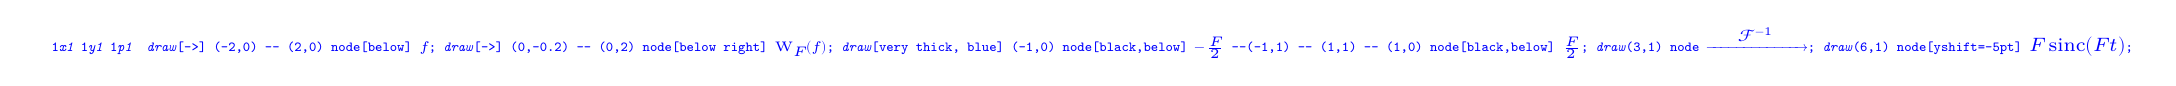
\begin{tikzpicture}
        \draw[->] (-2,0) -- (2,0) node[below] {$f$};
        \draw[->] (0,-0.2) -- (0,2) node[below right] {$\mathrm W_F(f)$};

        \draw[very thick, blue]
        (-1,0) node[black,below] {$-\frac{F}{2} $}
        --(-1,1) -- (1,1) -- (1,0) node[black,below] {$\frac{F}{2} $};

        \draw (3,1) node {\(
        	\xrightarrow{\qquad
        		\mathlarger{\mathlarger{\mathlarger{\mathscr F^{-1}}}}\qquad
        	}
        	\)};

        \draw (6,1) node[yshift=-5pt] {\(
        	\mathlarger{\mathlarger{\mathlarger{F\;\mathrm{sinc}(Ft)}}}
        	\)};


        \end{tikzpicture}

    \subsubsection{Δειγματοληψία}
    \begin{tikzpicture}
    \draw[thick] (0,0) circle(0.15);
    \fill[thick] (0,0) circle (0.03);

    \draw[snake,->] (0,2) node[right] {γινόμενο} -- (0,0.15);
    \draw[thick,->] (-2,0) -- ++(1.85,0) node[above,midway] {$g(t)$};
    \draw[thick,->] (0,-2) node[below] {$S_{T_S}$} -- ++(0,1.85);
    \draw[thick,->] (0.15,0) -- (2,0) node[below] {$g_s(T)$};

    \draw[->] (3,0) -- ++(1.5,0) node[above,midway] {$\mathscr F$};

    \begin{scope}[xshift=7cm]
    \draw[thick] (0,0) node {$*$} circle(0.15);

    \draw[snake,->] (0,2) node[right] {συνέλιξη} -- (0,0.15);
    \draw[thick,->] (-2,0) -- ++(1.85,0) node[above,midway] {$G(f)$};
    \draw[thick,->] (0,-2) node[below] {$F_P S_{F_P}$} -- ++(0,1.85);
    \draw[thick,->] (0.15,0) -- (2,0) node[below] {$G^S(f)$};

    \end{scope}

    \draw (0,-3) node {Δειγματοληψία};
    \end{tikzpicture}
    \begin{align*}
    G^S(f) &= G(f) * F_p S_{F_p}(f)
    \\ &= F_p G(f) * \left( \sum_n \delta(f-nF_p) \right)
    \\ &= F_p \sum_n G(f-nF_P)
    \end{align*}
    Παρατηρούμε τις επικαλύψεις μεταξύ των διαδοχικών φασμάτων (aliasing). Για να περιοριστεί
    αυτό μπορούμε να αυξήσουμε το \( F_p \) (\( \implies \) να αυξήσουμε τη συχνότητα
    δειγματοληψίας)

    \begin{tikzpicture}
    \draw[very thick,blue] plot [variable=\x,domain=-2:2,smooth,samples=20]
    ({\x}, {  1.5*exp( -\x*\x)   });

    \draw[->] (0,-0.5) -- (0,2) node[right] {$G(f)$};
    \draw[->] (-2,0) -- (2,0) node[below] {$f$};

    \draw (0,1.5) node[above left] {$A$};

    \draw[->,thick] (2,1) -- ++(2,0) node[above,midway] {After};

    \begin{scope}[xshift=7cm]
    \draw[very thick,blue!15]
    plot [variable=\x,xshift=2cm,domain=-2:2,smooth,samples=20]
    ({\x}, {  1.5*exp( -\x*\x)   });
    \draw[very thick,blue!40]
    plot [variable=\x,xshift=-1cm,domain=-2:2,smooth,samples=20]
    ({\x}, {  1.5*exp( -\x*\x)   });
    \draw[very thick,blue!40]
    plot [variable=\x,xshift=1cm,domain=-2:2,smooth,samples=20]
    ({\x}, {  1.5*exp( -\x*\x)   });
    \draw[very thick,blue] plot [variable=\x,domain=-2:2,smooth,samples=20]
    ({\x}, {  1.5*exp( -\x*\x)   });


    \draw[->] (0,-0.5) -- (0,2) node[right] {$G^S(f)$};
    \draw[->] (-2,0) -- (2.5,0) node[above right] {$f$};

    \draw (0,1.5) node[above left] {$A_{F_p}$};
    \draw (-1,0) node[below] {$-F_P$};
    \draw (1,0) node[below] {$F_P$};
    \draw (2,0) node[below] {$2F_P$};
    \end{scope}

    \end{tikzpicture}

    \begin{tikzpicture}[scale=1.1]

    \draw[very thick,blue] plot[smooth,tension=2] coordinates {(-1,0) (0,1.5) (1,0)};
    \draw (-1,0) node[below] {$-\sigma$};
    \draw (1,0) node[below] {$\vphantom{-} \sigma$};

    \draw (0,-1) node {$\sigma$-ζωνοπερατό};

    \draw[->] (0,-0.5) -- (0,2) node[right] {$G(f)$};
    \draw[->] (-2,0) -- (2,0) node[below] {$f$};

    \draw (0,1.5) node[above left] {$A$};
    \filldraw (0,1.5) circle (1pt);

    \draw[->,thick] (1.8,1) -- ++(2,0) node[above,midway] {After};

    \begin{scope}[xshift=8cm]
    \foreach \x in {-3,-1.5,...,1.5} {
    	\begin{scope}
    	\clip plot[xshift=\x cm,smooth,tension=2] coordinates {(-1,0) (0,1.5) (1,0)};
    	\fill[purple!40,postaction={pattern=north east lines,opacity=.2}]
    	plot[xshift={\x cm+1.5 cm},smooth,tension=2] coordinates {(-1,0) (0,1.5) (1,0)};
    	\end{scope}
    }

    \draw[xshift=3cm,very thick,blue!70,path fading=east]
    plot[smooth,tension=2] coordinates {(-1,0) (0,1.5) (1,0)};
    \draw[xshift=1.5cm,very thick,blue!85]
    plot[smooth,tension=2] coordinates {(-1,0) (0,1.5) (1,0)};
    \draw[xshift=-3cm,very thick,blue!70,path fading=west]
    plot[smooth,tension=2] coordinates {(-1,0) (0,1.5) (1,0)};
    \draw[xshift=-1.5cm,very thick,blue!85]
    plot[smooth,tension=2] coordinates {(-1,0) (0,1.5) (1,0)};
    \draw[very thick,blue] plot[smooth,tension=2] coordinates {(-1,0) (0,1.5) (1,0)};

    \draw[->] (0,-0.5) -- (0,2);
    \draw[->] (-3,0) -- (3,0);

    \draw[dashed] (1.5,1.5) -- ++(0,-1.5) node[below] {$F_P$};
    \draw[->] (0.5,-0.05) -- (0.5,-0.4) node[below] {$\mathsmaller{F_P-\sigma}$};

    \begin{scope}[yshift=-4cm]
    \fill[green!30,postaction={pattern=north west lines,opacity=.1}]
    (-1.3,0.7) rectangle (1.3,0);
    \draw[xshift=5cm,very thick,blue!70,path fading=east]
    plot[smooth,tension=2] coordinates {(-1,0) (0,1.5) (1,0)};
    \draw[xshift=2.5cm,very thick,blue!85]
    plot[smooth,tension=2] coordinates {(-1,0) (0,1.5) (1,0)};
    \draw[xshift=-5cm,very thick,blue!70,path fading=west]
    plot[smooth,tension=2] coordinates {(-1,0) (0,1.5) (1,0)};
    \draw[xshift=-2.5cm,very thick,blue!85]
    plot[smooth,tension=2] coordinates {(-1,0) (0,1.5) (1,0)};
    \draw[very thick,blue] plot[smooth,tension=2] coordinates {(-1,0) (0,1.5) (1,0)};

    \draw[->] (0,-0.5) -- (0,2);
    \draw[->] (-3,0) -- (3,0);

    \draw[dashed] (2.5,1.5) -- ++(0,-1.5) node[below] {$F_P$};
    \draw[->] (1.5,-0.05) -- (1.5,-0.4) node[below] {$\mathsmaller{F_P-\sigma}$};
    \draw[->] (3.5,-0.05) -- (3.5,-0.4) node[below] {$\mathsmaller{F_P+\sigma}$};

    \draw[green!50!black,very thick] (-1.3,0) -- ++(0,0.7)
    node[above,rotate=45,xshift=15pt,yshift=-1mm] {$W_F(f)$}
    -- ++(2.6,0) -- ++(0,-0.7);

    \draw[gray!50!black,thick,->] (0,-1) -- ++(0,-1);

    \draw[blue!50!black] (-1,0) node[below] {$-\sigma$};
    \draw[blue!50!black] (1,0) node[below] {$\vphantom{-} \sigma$};
    \end{scope}

    \begin{scope}[yshift=-8.5cm]
    \draw[->] (0,-0.5) -- (0,2);
    \draw[->] (-3,0) -- (3,0);

    \draw[very thick,blue] plot[smooth,tension=2] coordinates {(-1,0) (0,1.5) (1,0)};

    \draw[blue!50!black] (-1,0) node[below] {$-\sigma$};
    \draw[blue!50!black] (1,0) node[below] {$\vphantom{-} \sigma$};
    \end{scope}
    \end{scope}

    \end{tikzpicture}
    Για να μην έχουμε aliasing πρέπει:
    \[
    F_p -\sigma > \sigma \implies F_p > 2\sigma
    \]

    \[
    \text{\Large Nyquist's Criterion:} \quad \boxed{ \hspace{120pt}
    	\mathlarger{\mathlarger{\mathlarger{\mathlarger{\mathlarger{
    	\underbrace{F_p}_{\mathclap{\text{συχνότητα δειγματοληψίας}}} >
    	2\overbrace{\sigma}^{\mathclap{\text{max frequency}}}
    						}}}}} \hspace{100pt}
    	}
    \]

    \begin{center}
    \begin{tikzpicture}[scale=1.5]

    \fill[green!10,postaction={pattern=north west lines,opacity=.1}]
    (-1.7,0.7) rectangle (1.7,0);
    \draw[very thick,blue] plot[smooth,tension=2] coordinates {(-1,0) (0,1.5) (1,0)};

    \draw[->] (0,-0.5) -- (0,2) node[right] {$F_P-\sigma$};
    \draw (-3,0) -- (3,0);

    \draw[green!50!black,very thick] (-1.7,0) -- ++(0,0.7) -- ++(3.4,0) -- ++(0,-0.7);

    \draw (-1,0) node[below] {$-\sigma$};
    \draw (1,0) node[below] {$\vphantom{-} \sigma$};

    \draw[green!50!black] (-1.7,0) node[below] {$-\frac{F}{2}$};
    \draw[green!50!black] (1.7,0) node[below] {$\frac{F}{2}$};
    \end{tikzpicture}
    \end{center}
    \begin{gather*}
    W_F(f): \sigma < \sfrac{F}{2}  < F_p-\sigma \\
    \underbrace{F_p = W_F(f)\cdot G^S(f)}_{\downarrow ΙFT} \\
    F_p g(t) = \mathscr F^{-1} \left\lbrace W_F(f) \right\rbrace
    * \mathscr F^{-1} \left\lbrace G^S(f) \right\rbrace
    \end{gather*}
    \begin{align*}
    F_p g(t) &= F \sinc(Ft) * \left(
    \underbrace{g(t)\cdot S_{T_s}(t)}_{g_s(t)}
    \right) \\
    \\ &= F\int_{-\infty}^{\infty} g(t)\sum_n \delta(t'-nT_s)\sinc\left(F(t-t')\right)\dif t'
    \\ &= F\sum_n \int_{-\infty}^{\infty} g(t)\delta(t'-nT_s)\sinc\left(F(t-t')\right)\dif t'
    \\ &= \frac{F}{F_p} \sum_n g(nT_s) \sinc\left( F\cdot(t-nT_s) \right)
    \end{align*}

    \begin{align*}
    	g(kT_s) &= \frac{F}{F_P} \sum_n g(nT_s) \sinc\left(F(kT_s-nT_s)\right)
    	\\ F=F_p \qquad g(kT_s) &= \sum_n g(nT_s)\sinc(k-n)
    \end{align*}

    Γενικά, αν \(  F = F_p \):
    \[
    g(t) = \sum_n g(nT_s) \sinc\left( \frac{1}{T_s} (t-nT_s) \right)
    \]

	\paragraph[Δειγματοληψία όταν Fp=2σ]{Δειγματοληψία όταν \(F_p=2\sigma\)} \hspace{0pt}

    \begin{tikzpicture}

    \draw[very thick,blue] plot[variable=\x,domain=-2:3,smooth,samples=50]
    ({\x}, {  sin(\x r*pi/2*2)  });

    \draw[->] (0,-0.5) -- (0,2);
    \draw (-2,0) -- (3,0);

    \filldraw[very thick,draw=orange!60!black,fill=orange,fill opacity=.5]
    (0,0) circle (4pt) + (1,0) circle(4pt);

    \begin{scope}[yshift=-4cm,xshift=15pt]
    \draw[->] (0,-1.5) -- (0,2);
    \draw[->] (-2,0) -- (2,0);

    \draw[orange!70!black,ultra thick,->] (-1,0) -- ++(0,-1);
    \draw[orange!70!black,ultra thick,->] (1,0) -- ++(0,1);

    \begin{scope}[xshift=5cm]
    \draw[->] (0,-1.5) -- (0,2);
    \draw[->] (-2,0) -- (2.5,0);

    \draw[orange!70!black,ultra thick,->] (-1,0) -- ++(0,-1);
    \draw[orange!70!black,ultra thick,->] (1,0) -- ++(0,1);
    \draw[orange!70!black,ultra thick,->] (1,0) -- ++(0,-1);
    \draw[orange!70!black,ultra thick,->] (2,0) -- ++(0,1);

    \draw[orange!40!black,opacity=.5] (1,0) ellipse (0.5 and 1.5);

    \draw (1.5,1.5) node {$0$};
    \end{scope}
    \end{scope}
    \end{tikzpicture}

    Παρατηρούμε ότι οι \( \delta \) αφαιρούνται μεταξύ τους, οπότε \( G^S(f) = 0 \not\leftarrow
    \sin \), επομένως δεν μπορούμε να έχουμε \( F_p = 2\sigma \).

    \paragraph{Άσκηση για το σπίτι}
    \[
    \phi_n^{F,T_s}(t) = \sinc\left(  F(t-nF_p) \right)
    \]

    Να βρεθεί το \( \left\langle \phi_n(t),\phi_k(t)\right\rangle \).


    \subsection{Υποδειγματοληψία (undersampling)}
    
\begin{tikzpicture}[scale=2]
    \draw[very thick,red!50] (0.5,0) -- (0.5,1) -- (1.5,0);
    \draw[very thick,red!20] (-0.5,0) -- (-0.5,1) -- (0.5,0);
    \draw[very thick,red!10] (-1.5,0) -- (-1.5,1) -- (-0.5,0);

    \draw[very thick,green!70] (1.47,0) -- (1.47,1) -- (0.47,0);
    \draw[very thick,green!70] (3.5,0) -- (3.5,1) -- (2.5,0);
    \draw[very thick,green!40] (3.5,0) -- (3.5,1) -- (4.5,0);

    \draw[->] (-3,0) -- (5,0) node[below] {$f$};
    \draw[->] (0,-0.2) -- (0,2) node[right] {$x(f)$};

    \draw[very thick,blue] (1.5,0) node[black,below]
    {$f_L$} -- (1.5,1) -- (2.5,0) node[black,below] {$f_H$};



    \draw[very thick,blue] (-1.5,0) node[black,below]
    {$-f_L$} -- (-1.5,1) -- (-2.5,0) node[black,below] {$-f_H$};
    \end{tikzpicture}

    Για να μην πέφτουν τα "πλακάκια" το ένα πάνω στο άλλο:
    \begin{align*}
    \left. \begin{array}{ll}
    \kappa f_s-f_L < f_L \\
    (\kappa+1)f_s - f_H > f_H
    \end{array} \right\rbrace &\implies \begin{array}{l}
    f_s < \frac{2f_L}{\kappa} \\
    f_s > \frac{2f_H}{\kappa + 1}
    \end{array} \\
    &\frac{2f_H}{\kappa+1} < f_s < \frac{2f_L}{\kappa}
    \intertext{Ψάχνω το μέγιστο $\kappa$, έτσι ώστε να βρω το ελάχιστο $f_s$}
    \\& \frac{2f_H}{\kappa+1} < \frac{2f_L}{\kappa} \\ & k \leq \frac{f_L}{f_H-f_L}
    \\ \underset{\min}{f_s} \leftarrow & \kappa_{\text{best}} = \left\lfloor
    \frac{f_L}{f_H - f_L}
    \right\rfloor
    \end{align*}

    Θα ψάξω το ελάχιστο \( f_s \):
    \begin{gather*}
    	\frac{2f_H}{\left\lfloor\frac{f_L}{f_H-f_L}\right\rfloor+1} < f_s
    	< \frac{2f_L}{\left\lfloor\frac{f_L}{f_H-f_L}\right\rfloor} \\
    	\frac{2f_H}{\left\lfloor\frac{f_L}{f_H-f_L}+1\right\rfloor} < f_s
    	< \frac{2f_L}{\left\lfloor\frac{f_L}{f_H-f_L}+1\right\rfloor} \\
    	\frac{2f_H}{\left\lfloor\frac{f_H}{f_H-f_L}\right\rfloor} < f_s \\
    	\frac{2f_H}{\left\lfloor\frac{f_H}{f_H-f_L}\right\rfloor} =
    	\frac{2f_H}{\frac{f_H}{f_H-f_L}-\underset{\mathclap{0<\epsilon<1}}{\epsilon}}
    	=\frac{2f_H}{\frac{f_H-\epsilon f_H + \epsilon f_L}{f_H-f_L}}
    	= \frac{2f_H (f_H-f_L)}{f_H(1-\epsilon)+\epsilon f_L}
    	= \frac{2(f_H-f_L)}{(1-\epsilon)+\epsilon\frac{f_L}{f_H}} \\
    	= \frac{2(f_H-f_L)}{1-\epsilon\left(1-\frac{f_L}{f_H}\right)}
    	> 2(f_H - f_L) \quad \text{ αλλά όχι πολύ κοντά εκεί!}
    \end{gather*}
    \[
    2(f_H-f_L) < \boxed{
    	\frac{2f_H}{\left\lfloor\frac{f_L}{f_H-f_L}\right\rfloor + 1} < f_s
    	}
    \]

    
\begin{tikzpicture}[scale=1.5]
    \draw[thick,blue!50] (2,0) -- (2,1) --(1,0);
    \draw[thick,blue!50] (0,0) -- (0,1) -- (1,0);
    \draw[thick,blue!50] (-2,0) -- (-2,1) -- (-1,0);
    \draw[thick,blue!50] (0,0) -- (0,1) -- (-1,0);

    \filldraw[very thick,blue,fill=green!30] (2,0) node[black,below]
    {$f_L$} -- (2,1) -- (3,0) node[black,below] {$f_H$};
    \filldraw[very thick,blue,fill=green!30] (-2,0) node[black,below]
    {$-f_L$} -- (-2,1) -- (-3,0) node[black,below] {$-f_H$};

    \draw[->] (-4,0) -- (4,0) node[below] {$f$};
    \draw[->] (0,-0.2) -- (0,2) node[right] {$X^S(f)$};

    \draw[thick,green!60!black] (-3.05,0) -- ++(0,1.5) -- ++(1.1,0) -- ++(0,-1.5);
    \draw[thick,green!60!black] (3.05,0) -- ++(0,1.5) -- ++(-1.1,0) -- ++(0,-1.5);

    \draw[thick,orange!70] (-3.1,0) -- ++(0,3.5) -- ++(6.2,0) -- ++(0,-3.5);
    \draw[thick,red!70] (-1.9,0) -- ++(0,3) node[below left] {-} -- ++(3.8,0) -- ++(0,-3);

    \end{tikzpicture}

    \subsection{Gibbs' Phenomenon}
    \begin{tikzpicture}
    \draw (2.5,0) node[below] {$\vphantom{-}\sigma$} -- ++(0,{1.2*exp(-2.5^2/7)});
    \draw (-2.5,0) node[below] {$-\sigma$} -- ++(0,{1.2*exp(-2.5^2/7)});

    \fill[green!20] plot[variable=\x,domain=-2.5:2.5,smooth,samples=20]
    ({\x}, {  1.2*exp(-\x*\x/7)  }) -- (2.5,0) -- (-2.5,0) -- cycle;
    \draw[very thick,blue] plot[variable=\x,domain=-3:3,smooth,samples=20]
    ({\x}, {  1.2*exp(-\x*\x/7)  });

    \draw[->] (0,-0.5) -- (0,2) node[right] {$X(\omega)$};
    \draw[->] (-3,0) -- (3,0) node[right] {$\omega$};
    \end{tikzpicture}

    \begin{align*}
    x(t) &\xrightarrow{FT} X(\omega )
    \\ x_\sigma(t) &= \frac{1}{2\pi} \int_{-\sigma}^{\sigma}
    X(\omega ) e^{j\omega t} \dif\omega = \frac{1}{2\pi}
    \int_{-\sigma}^{\sigma} \boxed{\int_{-\infty}^{\infty} x(\tau) e^{j\omega\tau}\dif\tau }
    e^{j\omega t}\dif \omega
    \\ &= \frac{1}{2\pi} \int_{-\infty}^{\infty} x(\tau) \int_{-\sigma}^{\sigma}
    e^{-j\omega \tau +j\omega t}\dif\omega\dif t
    = \int_{-\sigma}^{\sigma} e^{j\omega (t-\tau)}\dif\omega
    \\ &= \left.\frac{1}{j(t-\tau)}e^{j\omega (t-\tau)} \right|_{-\sigma}^\sigma
    \\ &= \frac{1}{j(t-\tau)}\left[
    e^{j\sigma(t-\tau)}-e^{-j\sigma (t-\tau)}
    \right] \\ &= \frac{2}{t-\tau} \sin \left( \sigma(t-\tau) \right)
    \intertext{δηλαδή}
    X_\sigma(f) &= \int_{-\infty}^{\infty} x(\tau) \frac{\sin\left(\sigma(t-\tau)\right)}%
    {\pi(t-\tau)}\dif\tau
    \end{align*}

    \begin{tikzpicture}

    \draw[very thick,draw=blue]
    (-1,0) node[below] {$-\sigma$} -- (-1,1) -- (1,1) -- (1,0) node[below] {$\sigma$};
    \draw (0,1) node[above right] {$1$};


    \draw[->] (0,-0.5) -- (0,2) node[right] {$X(\omega)$};
    \draw[->] (-2,0) -- (2,0) node[right] {$\omega$};

    \draw[thick,->] (2,1) -- (3,1) node[midway,above] {IFT};
    \draw[thick,->] (0,-1) -- (0,-2) node[midway,right] {$\sigma\to\infty$};
    \draw[thick,->] (4,-1) -- (4,-2) node[midway,right] {$\sigma\to\infty$};

    \draw (4,1) node {$\mathlarger{\frac{\sin(\sigma t)}{\pi t}}$};

    \begin{scope}[yshift=-4.5cm]
    \draw[very thick,draw=blue] (-1.9,1) -- (1.9,1);


    \draw[->] (0,-0.5) -- (0,2) node[right] {$X(\omega)$};
    \draw[->] (-2,0) -- (2,0) node[right] {$\omega$};

    \draw[thick,->] (2.2,1) -- (3.2,1) node[midway,above] {IFT};

    \draw (4,1) node {$\mathlarger{\delta(t)}$};
    \end{scope}
    \end{tikzpicture}

    \begin{align*}
    	\lim_{\sigma\to \infty  }
    	x_\sigma(t) &= \int_{-\infty}^{\infty} x(\tau)
    	\lim_{\sigma\to \infty} \frac{\sin\left(\sigma(t-\tau)\right)}{\pi(t-\tau)}\dif\tau
    	\\ \lim_{\sigma\to \infty} x_\sigma(t) &=
    	\int_{-\infty}^{\infty} x(\tau)\delta(t-\tau)
    	\dif\tau \\
    	\lim_{\sigma \to \infty} x_\sigma(t) = x(t)
    \end{align*}

    \begin{tikzpicture}[scale=0.8]
    \draw[very thick,blue] plot[variable=\x,domain=-3:0,smooth,samples=40]
    ({\x}, {  0.4*sin(5*\x r)-\x  });
    \draw[very thick,blue] plot[variable=\x,domain=0:3,smooth,samples=40]
    ({\x}, {  1.5+0.3*sin(3*\x r)-\x/1.5  });

    \draw (0,0) node[below right] {$x(0^-)$};
    \draw (0,1.5) node[left,xshift=3pt] {$x(0^+)$};
    \draw[blue] (0.4,0.3) node[right] {$x(t)$};

    \draw[->] (0,-0.5) -- (0,2);
    \draw[->] (-3,0) -- (3,0) node[right] {$t$};

    \draw (4,1) node {$=$};

    \begin{scope}[xshift=7cm]
    \draw[very thick,blue] plot[variable=\x,domain=-3:0,smooth,samples=40]
    ({\x}, {  0.4*sin(5*\x r)-\x  });
    \draw[very thick,blue] plot[variable=\x,domain=0:3,smooth,samples=40]
    ({\x}, {  0.3*sin(3*\x r)-\x/1.5  });

    \draw (-2,1) node {$x(0^-)$};
    \draw (1.7,1) node {$x(0^-)$};

    \draw[->] (0,-0.5) -- (0,2) node[right] {$X_C(t)$};
    \draw[->] (-3,0) -- (3,0) node[right] {$t$};

    \draw (4,1) node {$+$};
    \end{scope}
    \begin{scope}[xshift=14cm]


    \draw[very thick,draw=blue,->] (0,0) -- (0,1.2)
    node[midway,above,xshift=10pt,sloped]
    {$\mathsmaller{\mathsmaller{\left[x(0^+)-x(0^-)\right]}}$}
    -- ++(3.2,0)
    node[midway,above] {$\left[x(0^+)-x(0^-)\right]\mathrm u(t)$};

    \draw (0,-0.5) -- (0,2);
    \draw[->] (-3,0) -- (3,0) node[right] {$t$};
    \end{scope}
    \end{tikzpicture}

    \begin{align*}
    x(t) &= x_c(t) + \left[x(0^+)-x(0^-)\right]\mathrm u(t)
    \\ x_\sigma(t) &= \int_{-\infty}^{\infty} x_c(t)
    \frac{\sin\left(\sigma(t-\tau)\right)}{\pi(t-\tau)}\dif\tau
    -\frac{\left[x(0^+)-x(0^-)\right]}{\pi} \int_{0}^{\infty}
    \frac{\sin\left(\sigma(t-\tau)\right)}{(t-\tau)}\dif \tau \\
    \int_0^\infty \frac{\sin\left(\sigma(t-\tau)\right)}{t-\tau}\dif\tau & \\
    \text{Θέτουμε }&\begin{array}{l}
    \sigma(t-\tau)=x \\ \dif\tau = -\frac{1}{\sigma}\dif x \\ t-\tau = \frac{x}{\sigma}
    \end{array}
    \\ &= \int_{\sigma t}^{\infty} \frac{\sin x}{\frac{x}{\sigma}} \left(
    \frac{\sin x}{x}\dif x
    \right) = \int_{-\infty}^{0} \frac{\sin x}{x}\dif x + \int_0^{\sigma t}\frac{\sin x}{x}
    \dif x
    \\ &= \frac{\pi}{2} + \int_{0}^{\sigma t} \frac{\sin x}{x}\dif x
    = \frac{\pi}{2} + \underbrace{\mathrm{Si}(\sigma t)}_{\mathclap{\text{Sine Integral}}}
    \end{align*}

    Άρα
    \begin{align*}
    	x_\sigma(t) &= \int_{-\infty}^{\infty} x_c(\tau)
    	\frac{\sin\left(\sigma(t-\tau)\right)}{\pi(t-\tau)}\dif\tau
    	+ \frac{\left[x(0^+)-x(0^-)\right]}{2}
    	+ \frac{\left[x(0^+)-x(0^-)\right]}{\pi} \cdot
    	\mathrm{Si}\; (\sigma t)
    \end{align*}

    \paragraph{}
    \[
    \mathrm{Si}(t) = \int_0^t \frac{\sin x}{x}\dif x
    \]

    \begin{tikzpicture}

    \draw[dashed,draw=brown!40!black]
    (0,pi/2) node[left] {$\frac{\pi}{2}$} -- ++(5,0);
    \draw[dashed,draw=brown!40!black]
    (0,-pi/2) node[right] {$-\frac{\pi}{2}$} -- ++(-4,0);

    \draw[dashed,brown!80!black] (0,{pi*(1/2+0.0895)}) -- ++(5,0);
    \draw[thick,<->] (4.5,pi/2) -- ++(0,0.0895*pi) node[midway,right,yshift=-1pt]
    {$\pi \cdot 0,0895\dots$};

    \draw[very thick,blue] plot[xscale={1/pi},smooth] file{data/sine_integral.data};


    \draw[->] (0,-2) -- (0,2);
    \draw[->] (-4,0) -- (4,0) node[right] {$t$};

    \draw (1,0.1) -- ++(0,-0.2) node[below] {$\frac{\pi}{\sigma}$};
    \draw (2,0.1) -- ++(0,-0.2) node[below] {$\frac{2\pi}{\sigma}$};
    \draw (3,0.1) -- ++(0,-0.2) node[below] {$\frac{3\pi}{\sigma}$};
    \draw (-1,0.1) -- ++(0,-0.2) node[below] {$\frac{-\pi}{\sigma}$};
    \draw (-2,0.1) -- ++(0,-0.2) node[below] {$\frac{-2\pi}{\sigma}$};
    \draw (-3,0.1) -- ++(0,-0.2) node[below] {$\frac{-3\pi}{\sigma}$};

    \draw (5,0) node {$\mathlarger{\mathrm{Si}\, (\sigma t)}$};

    \end{tikzpicture}

    Χρησιμοποιώντας τον Leibniz Rule (παραγωγίζοντας το ολοκλήρωμα) μπορούμε να αποδείξουμε
    την θέση των μεγίστων της \( \mathrm{Si} \).

    \begin{align*}
    	x_\sigma(t) &= \int_{-\infty}^{\infty} x_c(t)
    	 \frac{\sin\left[\sigma(t-\tau)\right]}{\pi(t-\tau)} \dif\tau +
    	 \frac{x(0^+)-x(0^-)}{2} + \frac{\left[x(0^+)-x(0^-)\right]}{\pi}\mathrm{Si}(\sigma t)
      \\ \lim_{\sigma\to \infty} x_\sigma(t) &= x_c(t) + \frac{x(0^+)-x(0^-)}{2}
      + \frac{\left[x(0^+)-x(0^-)\right]}{\pi} \lim_{\sigma\to \infty}\mathrm{Si}(\sigma t)
      \\ \lim_{\sigma\to \infty} x_\sigma(0) &= x(0^-) + \frac{x(0^+)-x(0^-)}{2}
      = \frac{x(0^+)+x(0^-)}{2}
    \end{align*}

    \begin{tikzpicture}

    \draw[ultra thick,red!90!blue] (-2,pi/2) -- (0,pi/2) -- (0,-pi/2) -- (2,-pi/2);

    \draw[thick,blue] plot[xscale={-0.5/pi},smooth] file{data/sine_integral.data};

    \filldraw[very thick, draw=brown!50!black, fill=orange, fill opacity=.8]
    (0,0) circle (4pt);

    \end{tikzpicture}

    Παρατηρώ ότι τα ζιγκζακωτά παραμένουν και το ύψος του κυματισμού δεν αλλάζει. Το μόνο που
    μπορεί να μεταβληθεί είναι η θέση του μεγίστου, με αύξηση του \( \sigma \) (ώστε να
    έρθει πιο κοντά στο σημείο ασυνέχειας). Αυτό είναι το φαινόμενο Gibbs.

    Εάν όμως το \( \sigma \) δεν τείνει στο \( \infty \), το αποτέλεσμα στο \( 0 \) δεν είναι
    απαραίτητα το ημιάθροισμα των \( x(0^+) \) και \( x(0^-) \).

    \subsection{Ευστάθεια συστήματος}
    Ευσταθές ονομάζεται ένα σύστημα όταν πεπερασμένη (φραγμένη στο πλάτος) είσοδος
    δίνει πεπερασμένη έξοδο -
    ΠΕΠΕ (Πεπερασμένη Είσοδος - Πεπερασμένη Έξοδος) / BIBO (Bounded Input - Bounded Output)
    ευστάθεια

    Φραγμένη συνάρτηση \( f(t) \in BF \) σημαίνει ότι
    \[
    \exists M>0 : \forall t \quad \left|f(t)\right| < M
    \]
    όπου \( BF \) ο κόσμος των φραγμένων συναρτήσεων.

    Ένα σύστημα είναι ευσταθές όταν \( \forall  \) είσοδο \( x(t) \in BF \) η έξοδος του
    συστήματος είναι επίσης φραγμένη (\( y(t) \in BF \)).
    (
    Αν το σύστημά μας είναι γραμμικό και ΑΚΜ (Αμετάβλητο Κατά τη Μετατόπιση)
    \[
    \exists h(t) \text{ κρουστική απόκριση }\quad y(t) = h(t)*x(t) = \int_{-\infty}^{\infty}
    h(\tau)x(t-\tau)\dif\tau
    \]

    Έστω \begin{align*}
    \exists M : \forall t,\quad & \left|x(t)\right| < M \implies
    \\& \left|x(t-\tau)\right| < M
    \end{align*}

    Επίσης έστω \begin{align*}
    	\exists N:& \left|y(t)\right| < N \quad \forall t
    	\\ & \left|y(t)\right| = \left|
    	\int_{-\infty}^{\infty} h(t) x(t-\tau)\dif \tau
    	\right| < \int_{-\infty}^{\infty} \left|h(t)x(t-\tau)\right|\dif\tau
    	< \int_{-\infty}^{\infty} \left|h(\tau)\right|\dif\tau < \frac{N}{M}
    \end{align*}

    Εάν η κρουστική απόκριση είναι απολύτως ολοκληρώσιμη, τότε το σύστημα είναι ευσταθές.

    \subsection{Ιδανικό φίλτρο}
    Έστω ένα ιδανικό χαμηλοπερατό φίλτρο:

    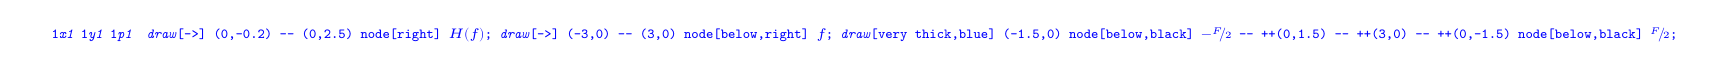
\begin{tikzpicture}
        \draw[->] (0,-0.2) -- (0,2.5) node[right] {$H(f)$};
    	\draw[->] (-3,0) -- (3,0) node[below,right] {$f$};

    	\draw[very thick,blue] (-1.5,0) node[below,black] {$-\sfrac{F}{2}$}
    	-- ++(0,1.5) -- ++(3,0) -- ++(0,-1.5) node[below,black] {$\sfrac{F}{2}$};
    \end{tikzpicture}

    \[
    W_F(f) \xrightarrow{\text{IFT}} h(t) = F\sinc (Ft) = F \frac{\sin(\pi Ft)}{\pi Ft}
    \]

    \begin{tikzpicture}[scale=1.2]
    \filldraw[xscale=0.5,samples=200,domain=-5:5,smooth,variable=\x,blue,
    fill=blue!20]
    plot ({\x},{abs(sinc(pi*\x))});

    \draw[->] (0,-0.5) -- (0,1.5) node[right] {$h(t)$};
    \draw[->] (-2.5,0) -- (2.5,0) node[below,right] {$t$};

    \draw[very thick,xscale=0.5,samples=200,domain=-5:5,smooth,variable=\x,blue]
    plot ({\x},{sinc(pi*\x)});

    \draw (0,0) node[below right] {$0$};
    \draw (0.5,0) node[below] {$\frac{1}{F}$};
    \draw(1,0) node[below] {$\frac{2}{F}$};
    \draw(1.5,0) node[below] {$\frac{3}{F}$};
    \draw (-0.5,0) node[below] {$-\frac{1}{F}$};
    \draw(2,0) node[below] {$\cdots$};
    \end{tikzpicture}

    Παρατηρώ ότι η κρουστική απόκριση του ιδανικού αυτού φίλτρου δεν είναι αιτιατή, οπότε ένα
    τέτοιο φίλτρο δεν είναι υλοποιήσιμο.

    Άσκηση για το σπίτι: Η \( h(t) \) είναι απολύτως ολοκληρώσιμη;

    \subparagraph{Απάντηση}
    \begin{tikzpicture}[baseline=(current bounding box.north)]

    \filldraw[xscale=0.8,samples=200,domain=-3:3,thick,variable=\x,blue,
    fill=blue!20]
    plot ({\x},{  abs(sinc(pi*\x))  });
    \filldraw[xscale=0.8,samples=25,domain=-1:1,smooth,thick,variable=\x,blue,
    fill=blue!30]
    plot ({\x},{  abs(sinc(pi*\x))  });

    \draw (0,-0.5) -- (0,1.5) ;
    \draw[->] (-2.5,0) -- (2.5,0) node[below,right] {$t$};


    \draw (0.8,0) node[below] {$k$};
    \draw (1.6,0) node[below] {$k+1$};
    \draw (0,0.5) node[right] {$\Xi$};
    \end{tikzpicture}

    \begin{gather*}
    \int_0^\pi \sin(t) \dif t = 2
    k \leq t \leq k+1 \quad \left|h(t)\right| = \left|\frac{\sin(t)}{t}\right| >
    \frac{\left|\sin(t)\right|}{k+1} \\
    \int_1^\infty \left|h(t)\right|\dif t > \sum_{k=1}^\infty \int_k^{k+1}
    \left|\frac{\sin(t)}{t}\right|\dif t > \sum_{n=1}^\infty \frac{1}{k+1}
    \cancelto{2}{\int \left|\sin(t)\right|} \\
    \int_{-\infty}^{\infty} \left|h(t)\right|\dif t > \Xi + 2\sum_{k=1}^\infty
    \frac{2}{k+1}
    \end{gather*}
    Δηλαδή το σύστημα του ιδανικού χαμηλοπερατού φίλτρου δεν είναι ευσταθές.

    \subsection{Kramers - Kronig}
    Έστω \( h(t) \) αιτιατή - πραγματική συνάρτηση με Μ\( F \): \( H(\omega )=
    H_R(\omega ) + jH_I(\omega ) \)

    \begin{gather*}
\text{Ξέρω }    h(t) = \underbrace{h_e(t)}_{\mathclap{\text{even}}} +
    \underbrace{h_o(t)}_{\mathclap{\text{odd}}} \\
\text{Ξέρω }    h_o(t) \xrightarrow{\text{FT}} H_o(\omega ) \in \mathbb I \quad
\text{(επίσης περιττή συνάρτηση)}\\
\text{Ξέρω }    h_e(t) \xrightarrow{\text{FT}} H_e(\omega ) \in \mathbb R \quad
\text{(επίσης άρτια συνάρτηση)}
    \end{gather*}
    \begin{gather*}
    h_o(t) = -h_e(t) \quad t<0 \\
    h_0(t) = h_e(t) \quad t \geq 0 \\
    \text{Συνεπώς } h(t) = h_e(t) + \mathrm{sgn}(t) h_e(t) \\
    \text{        } h(t) = h_o(t) + \mathrm{sgn}(t) h_o(t)
    \end{gather*}
    \begin{gather*}
    X(\omega ) = \int_{-\infty}^{\infty} x(t)e^{-j\omega t}\dif t \\
    x_1(t) x_2(t) \xrightarrow{\text{FT}} \frac{1}{2\pi}X_1(\omega )*X_2(\omega ) \\
    \mathrm{sgn}(t) \xrightarrow{\text{FT}} \frac{2}{j\omega } \\
    h(t) = h_e(t) + \mathrm{sgn}(t) h_e(t) \xRightarrow{\text{FT}}
    H(\omega ) = H_e(\omega ) + \frac{1}{2\pi}\frac{2}{j\omega }*H_e(\omega )
    = H_e(\omega ) - j\frac{1}{\pi} \int_{-\infty}^{\infty} \frac{1}{\omega -\omega'}
    H_e(\omega')\dif \omega' \\
    \boxed{
    	H(\omega ) = \underbrace{H_e(\omega ) }_{H_R(\omega )}
    	- \underbrace{j\frac{1}{\pi}\int_{-\infty}^{\infty}
    	\frac{H_e(\omega' )}{\omega -\omega'}\dif \omega' }_{jH_I(\omega )}
    	}
    \\ \boxed{
    	H_I(\omega ) = -\frac{1}{\pi}
    	\int_{-\infty}^{\infty} \frac{H_R(\omega')}{\omega -\omega'}\dif \omega'
    	}
    \end{gather*}
    ομοίως από πάνω υπολογίζουμε το \( H_R \).

   \section{Συστήματα}

   \subsection{Ανακεφαλαίωση}
   \paragraph{Γραμμικά Αναλογικά Συστήματα}
   \begin{enumerate}
   	\item \underline{Γραμμικότητα }
   	\qquad \( T\left[ax_1(t)+bx_2(t)\right] = ay_1(t)+by_2(t) \)
   	όπου \( \begin{array}{l}
   	y_1(t) = T\left[x_1(t)\right] \\
   	y_2(t) = T\left[x_2(t)\right]
   	\end{array} \qquad \forall x_1(t),x_2(t),\ a,b\)
   	\item \underline{Χρονοαμετάβλητο}
   	\qquad \( T\left[x(t-k)\right] = y(t-k) \)
   	όπου \( y(t)=T\left[x(t)\right] \qquad \forall k,x(t) \)
   	\item \underline{\textbf{Στιγμιαίο} (\( \neq \) δυναμικό)}
   	\qquad \( y(t) = f\left(x(t)\right) \)

   	Η έξοδος οποιαδήποτε χρονική στιγμή \( t \) εξαρτάται μόνο από την είσοδο την ίδια
   	στιγμή \( t \).

   	Η αντίσταση είναι ένα στιγμιαίο σύστημα, ενώ ο πυκνωτής και το πηνίο δεν είναι.
   	\item \underline{Αιτιατό} \qquad
   	Η έξοδος δεν εξαρτάται από μελλοντικές τιμές της εισόδου
   	\[ \left[\begin{matrix}
   	\text{\small ΞΕΡΩ} \\ \text{\small Γραμμικό} \\ \text{\small Χρον. Αμετάβλητο}
   	\end{matrix}\right] \implies h(t) = 0 \quad \forall t < 0 \]

   	\item \underline{Ευσταθές} \qquad
   	Για κάθε φραγμένη είσοδο, η έξοδος είναι φραγμένη.
   	\[ \left[\begin{matrix}
   	\text{\small ΞΕΡΩ} \\ \text{\small Γραμμικό} \\ \text{\small Χρον. Αμετάβλητο}
   	\end{matrix}\right] \implies \int_{-\infty}^{\infty} \left|h(t)\right|\dif t
   	< \infty \]

   	\item \underline{Συγκεντρωμένο και Κατανεμημένο}
   	\qquad Συγκεντρωμένο λέγεται όταν μοναδική ελεύθερη μεταβλητή είναι ο χρόνος \( t \).
   \end{enumerate}

   \paragraph{Παράδειγμα} Το σύστημα \( y(t) = x^2(t) \) είναι:
   \begin{enumerate}[itemsep=-1mm]
   	\item Μη γραμμικό
   	\item Χρονοαμετάβλητο
   	\item Στατικό (στιγμιαίο)
   	\item Αιτιατό
   	\item Ευσταθές
   	\item Συγκεντρωμένο
   \end{enumerate}

   \subsection{Περιγραφή συστήματος με διαφορική εξίσωση}
   \[
   \sum_{i=0}^{n} a_i \od[i]{}{t} y(t) = \sum_{l=0}^m b_l \od[l]{}{t}x(t) \qquad
   t \geq 0
   \]
   \begin{enumerate}[itemsep=-.5mm]
   	\item Γραμμικό
   	\item Χρονοαμετάβλητο
   	\item Δυναμικό, εκτός αν \( n=m=0 \)
   	\item Αιτιατό
   \end{enumerate}

   \begin{align*}
   	\text{Ολική λύση } &= \text{Ομογενής $+$ Μερική Λύση}\\
   	\text{Ολική λύση } &= \underbrace{\text{Εξαναγκασμένη λύση }}_{\text{%
   			λύση θεωρώντας δεδομένη $x(t)$ και μηδενικές Α.Σ.}} +
   	\underbrace{\text{Ελεύθερη λύση}}_{\text{Λύση θεωρώντας $x(t)$=0 και δεδομένες Α.Σ.}}
   	\intertext{(Τα ζευγάρια ομογενής/ελεύθερη \& εξαναγκασμένη/μερική δεν ταυτίζονται!)}
   	\text{Ολική λύση } &= \text{Λύση μόνιμης κατάστασης $+$ μεταβατική λύση}
   \end{align*}

   \paragraph{Μ. Laplace}
   \[
   \int_{i=0}^n a_i\left(
   s^i Y(s) - \sum_{k=0}^{i-1} s^{i-k-1}y_0^{(k)}
   \right) = \int_{l=0}^m b_l\left(
   s^i X(s) - \sum_{k=0}^{l-1} s^{l-k-1}x_0^{(k)}
   \right)
   \]
   \begin{gather*}
   Y(s) = \underbrace{\dfrac{\sum_{l=0}^m b_ls^l}{\sum_{i=0}^n a_is^i} X(s)
   - \dfrac{\sum_{l=0}^m\sum_{k=0}^{l-1} b_l s^{l-k-1}x_0^{(k)}}{\sum_{i=0}^n a_is^i}}_%
{\mathclap{\text{εξαναγκασμένη}}}
   + \underbrace{\dfrac{\sum_{i=0}^n \sum_{k=0}^{l-1} a_i s^{i-k-1}y_0^{(k)}}%
   	{\sum_{i=0}^n a_is^i}}_{\mathclap{\text{ελεύθερη}}}
   \end{gather*}

   \subparagraph{}
   \begin{align*}
   	y(t) &= x(t)*h(t) \\ Y(s) &= X(s)H(s)
   \end{align*}

   Συγκρίνοντας με τον παραπάνω τύπο, παρατηρούμε ότι η \( y(t)=x(t)*h(t) \) μόνο\
   όταν οι αρχικές συνθήκες είναι 0!

   \paragraph{Μ. Fourier}
   Για να λύσω το σύστημα \( \forall t > 0 \), θα πρέπει να μετασχηματίσω το αιτιατό κομμάτι
   του συστήματος μόνο:

   \( x_1(t) = x(t)\mathrm u(t) \)

   \( y_1(t) = y(t)\mathrm u(t) \)

   Άρα:
   \begin{gather*}
   	\od{x_1}{t} = \od{x}{t}\mathrm u(t) + x(0)\delta(t) \\
   	\od{y_1}{t} = \od{y}{t}\mathrm u(t) + y(0)\delta(t) \\
   	\od[i]{y_1(t)}{t} = \od[i]{y}{t}\mathrm u(t) + \sum_{k=0}^{i-1} y_0(k)
   	\delta(\tau)^{(\tau -1 -k)}
   	\\
   	\od[i]{x_1(t)}{t} = \od[i]{x}{t}\mathrm u(t) + \sum_{k=0}^{l-1} x_0(k)
   	\delta(\tau)^{(i -1 -l)} \\
   	\sum_{i=1}^N a_i\od[i]{y_1}{t} = \sum_{l=0}^{m} b_l\od[l]{x_1}{t}
   \end{gather*}

   Τελικά προκύπτει ότι η λύση της διαφορικής εξίσωσης \( y_1 \) που μας ενδιαφέρει είναι:
   \[
   y_1(t) = \mathrm{IFT} \left\lbrace
   \frac{\sum_{l=0}^m \log(j\omega )^l}{\sum_{i=0}^{n} a_i(j\omega)^i}X_1(\omega )
   -\frac{\sum_{l=0}^{m}\sum_{k=0}^{l-1} b_l(j\omega)^{l-k-1}x_0^{(k)}}{\sum_{i=0}^{n}
   	a_i(j\omega)^i}
   +\frac{\sum_{i=0}^{n}\sum_{k=0}^{i-1}
   	a_i(j\omega )^{i-1-k} y_0^{(k)}
   	}{\sum_{i=0}^n a_i(j\omega )^i}
    \right\rbrace
   \]

   Για την έξοδο σε ένα αιτιατό σύστημα θα χρησιμοποιώ Μ/Σ Laplace.

   Για μελέτη στη μόνιμη κατάσταση (\( t \to \infty \)), όπου οι αρχικές συνθήκες δεν
   συνεισφέρουν, θα χρησιμοποιώ Μ/Σ Fourier, παίρνοντας τον μετασχηματισμό όλης της συνάρτησης
   και όχι μόνο του αιτιατού μέρους της.

   \paragraph{Ex.1} \mbox{} \\
   \begin{circuitikz} \draw
   	(0,0) to[battery1=$v$,i_=$i$] (0,2)
   	to[switch] (2,2)
   	to[R=$R$,i] (4,2)
   	to[C=$C_Q$,v=$V_0$] (4,0) -- (0,0);
   \end{circuitikz}

   \begin{align*}
   	v(t) &= Ri(t) + \frac{1}{c} \int_0^t i(\tau)\dif\tau + V_0\mathrm u(t) \\
   	V(s) &= RI(s) + \frac{1}{C}\frac{I(s)}{s}+\frac{V_0}{s} \\
   	\xrightarrow{V_0=0} H(s) &= \frac{I(s)}{V(s)} = \frac{1}{R+\frac{1}{Cs}}
   	= \frac{Cs}{RCs+1}\cdot \frac{\sfrac{S}{R} }{\sfrac{S+1}{RC} }
   	\\ &= \frac{1}{R} \left(1-\frac{\sfrac{1}{RC} }{s+\sfrac{1}{RC} }\right)
   	\\ H(\omega ) &= \frac{1}{R} \left(1-\frac{\sfrac{1}{RC} }{j\omega+\sfrac{1}{RC} }\right)
   	\\ h(t) &= \mathrm{ILT}\left\lbrace H(s) \right\rbrace
   	= \frac{1}{R}\delta(t) - \frac{1}{R^2 C}e^{-\frac{1}{RC}t}\mathrm u(t)
   \end{align*}

   Έξοδος \( i(t) = h(t) * V(t) = \left[\frac{1}{R}\delta(t)
   -\frac{1}{R^2 C}e^{-\sfrac{1}{RC}\cdot t }
   \right]*\left[V\mathrm u(t)\right] = \cdots = \frac{V}{R}e^{-\sfrac{t}{RC}\mathrm u(t)} \)

   Επειδή όμως οι αρχικές συνθήκες δεν είναι μηδενικές (ο πυκνωτής είναι φορτισμένος),
   το παραπάνω αποτέλεσμα είναι λάθος!

   Η σωστή λύση είναι:
   \begin{align*}
   	v(t) &= Ri(t)+\frac{1}{C}\int_0^t i(\tau)\dif\tau + V_0 \mathrm u(t) \\
   	V(s) &= RI(s) + \frac{1}{C}\frac{I(s)}{s}+\frac{V_s}{s} \\
   	I(s) \left[R+\frac{1}{Cs}\right] &= V(s) - \frac{V_0}{s} \\
   	I(s) &= \frac{V(s) -\sfrac{V_0}{s} }{R+\frac{1}{Cs}} = \frac{(V-V_0)}{s}\cdot
   	\underbrace{\frac{1}{R+\frac{1}{Cs}}}_{H(s)} \\
   	i(t) &= \frac{V-V_0}{R}e^{\sfrac{-t}{RC}}\mathrm u(t)
   	\\ &= \underbrace{
   		\underbrace{\frac{V}{R}e^{\sfrac{-t}{RC}}}_{\mathclap{\text{εξαναγκασμένη λύση}}}
   		- \frac{V_0}{R}e^{\sfrac{-t}{RC}}}_%
   	{\mathclap{\text{μεταβατική λύση}}}
   \end{align*}

    \subsection{Decibels (dB)}
    Έστω
    \begin{align*}
    	x_A(t) &= A\sin(\omega_1 t) \\
    	y_B(t) &= B\sin(\omega_1 t)
    \end{align*}

    \begin{gather*}
    	x_Α \text{ πλάτος } A > 0 \\
    	x_B \text{ πλάτος } B > 0 \\
    	\boxed{\mathrm{dB} = 20\log_{10} \frac{A}{B}}
    \end{gather*}

    \paragraph{Για την ισχύ:}
    \begin{gather*}
    c\cdot x_Α^2 \text{ ισχύς } A \\
    c\cdot x_B^2 \text{ ισχύς } B \\
    \boxed{\mathrm{dB} = 10\log_{10} \frac{A^2}{B^2}}
    \end{gather*}

    Παρατηρούμε ότι τα dB πλάτους και dB ισχύος είναι το ίδιο!

    \begin{tikzpicture}
    \draw[->] (-3,0) -- (3,0) node[right] {$\omega$};
    \draw[->] (0,-0.7) -- (0,2.5) node[right] {$H(\omega)$};

    \draw[dashed] (0.79,0) node[below] {$\omega_1$} -- ++(0,1.83) -- ++(-0.79,0);

    \draw[very thick, blue] plot [smooth] coordinates {
    	(-2,0) (-1.5,1.7) (1.5,1.7) (2,0)};

    \begin{scope}[yshift=-4cm]
    \draw[->] (-3,0) -- (3,0) node[right] {$\omega$};
    \draw[->] (0,-0.7) -- (0,2.5) node[right] {$\mathrm{dB}$};

    \draw (0,0) node[below left] {$0$};
    \draw[dashed] (.79,0) node[below] {$50$Hz} -- ++(0,1) -- (0,1) node[left] {$3$};

    \draw[very thick,samples=100,yscale=1.8,domain=-3:2.96,smooth,variable=\x,blue]
    plot ({\x},{exp(-\x*\x)});
    \end{scope}

    \end{tikzpicture}


    \( \pm 3\mathrm{dB} \) σημαίνει (υπο)διπλασιασμό της ισχύος, ή
    πολλαπλασιασμό/διαίρεση του πλάτους με \( \sqrt{2} \).


   \section{Ασκήσεις}
   \paragraph{Άσκηση} \( x(t) = 4000\sinc(4000t) \)
   \begin{enumgreekparen}
   	\item \( X(f) = ? \)
   	\item Nyquist Συχνότητα για τα \( x(t) \) και \( x^2(t) \)
   \end{enumgreekparen}

   \begin{enumgreekparen}
   	\item
   	
\begin{tikzpicture}[baseline=(current bounding box.north)]
   	\draw[->] (-3,0) -- (3,0) node[below right] {$f (\mathrm{Hz})$};
   	\draw[->] (0,-0.7) -- (0,2);

   	\draw[very thick, blue] (-2,0) -- (-2,1.2) -- (2,1.2) -- (2,0);
   	\draw (-2,0) node[below] {$\sfrac{-T}{2} $};
   	\draw (2,0) node[below] {$\sfrac{T}{2} $};
   	\draw (0,1.2) node[above right] {$1$};

   	\draw[->] (4,0.5) -- ++(2,0)
   	node[above,midway] {FT} node[below,midway] {$f$};
   	\draw (7,0.5) node {$\mathlarger{T\sinc(Tf)}$};

   	\draw[->] (3.5,1) node[left] {$\mathrm W_T(t)$} to[bend left=45] (6.5,1);

   	\end{tikzpicture}

    \begin{gather*}
    	T\sinc(Tt) \xrightarrow{\text{FT}} \mathrm W_T (f) \\
    	x(t) = 4000\sinc (4000t) \xrightarrow[f]{\text{FT}}
    	W_{4000}(f) = 
\begin{tikzpicture}[baseline=-0.65ex,scale=0.5]
    	\draw[->] (-3,0) -- (3,0) node[below right] {$f (\mathrm{Hz})$};
    	\draw[->] (0,-0.7) -- (0,2);
    	\draw[very thick, blue] (-2,0) -- (-2,1.2) -- (2,1.2) -- (2,0);
    	\draw (-2,0) node[below] {$-2000$};
    	\draw (2,0) node[below] {$2000$};
    	\draw (0,1.2) node[above right] {$1$};
    	%\draw (4, .5) node
    	%{$\mathlarger{\mathlarger{\mathlarger{\mathlarger{\mathlarger{*}}}}}$};
    	\end{tikzpicture}
    \end{gather*}
    \item Nyquist συχνότητα για το \( x(t) \) είναι \( 2\times 2000\ \mathrm{Hz}
    = 4000\ \mathrm{Hz}
     \)

     \[
     \mathrm{FT}\left\lbrace x^2(t) \right\rbrace
     = \mathrm{FT}\left\lbrace x(t)x(t) \right\rbrace
     = X(f) * X(f)
     \]

     \begin{tikzpicture}[scale=0.7]
     \draw (-3,0) -- (3,0);
     \draw (0,-1) -- (0,2);

     \draw[very thick, blue] (-2,0) -- (-2,1.3) -- (2,1.3) -- (2,0);
     \draw (-2,0) node[below] {$-2\mathrm{k}$};
     \draw (2,0) node[below] {$2\mathrm{k}$};

     \draw (4, .5) node
     {$\mathlarger{\mathlarger{\mathlarger{\mathlarger{\mathlarger{*}}}}}$};

     \begin{scope}[xshift=8cm]
     \draw (-3,0) -- (3,0);
     \draw (0,-1) -- (0,2);

     \draw[very thick, blue] (-2,0) -- (-2,1.3) -- (2,1.3) -- (2,0);
     \draw (-2,0) node[below] {$-2\mathrm{k}$};
     \draw (2,0) node[below] {$2\mathrm{k}$};
     \end{scope}

     \draw (12, .5) node
     {$\mathlarger{\mathlarger{\mathlarger{\mathlarger{\mathlarger{=}}}}}$};

     \begin{scope}[xshift=16cm]
     \draw (-3,0) -- (3,0);
     \draw (0,-1) -- (0,2);

     \draw[very thick, blue] (-2.5,0) -- (0,1.3) -- (2.5,0);
     \draw (-2.5,0) node[below] {$-4\mathrm{k}$};
     \draw (2.5,0) node[below] {$4\mathrm{k}$};
     \end{scope}

     \end{tikzpicture}

     Για το \( x^2(t) \) η Nyquist είναι \( 2\cdot 4\ \mathrm{kHz} = 8\ \mathrm{kHz} \)
   \end{enumgreekparen}

   \paragraph{Άσκηση} \hspace{0pt}

   
\begin{tikzpicture}
   \draw[->] (0.25,0) -- (2-.2,0) node[above,midway] {$x(t)$};

   \draw[->] (2,0) -- ++(0,-3) -- ++(1.5,0) node[midway,above] {$a$} -- ++(0,0.75);
   \draw (3,-2.25) rectangle ++(1,1.5) node[midway]
   {$\mathlarger{\mathlarger{\mathlarger{\int}}}$};
   \draw[->] (3.5,-0.75) -- (3.5,-0.25);
   \draw (3.5,-0.25) -- (3.5, 0);

   \draw[->] (5.5,-2.25) -- (5.5,-3);
   \draw[->] (5.5,-3) -- ++(1.5,0) node[midway,above] {$b$} -- ++(0,3-.2);
   \draw (5,-2.25) rectangle ++(1,1.5) node[midway]
   {$\mathlarger{\mathlarger{\mathlarger{\int}}}$};
   \draw (5.5,-0.75) -- (5.5,-0.25);
   \draw[<-] (5.5,-0.35) -- (5.5, 0);

   \draw[<->] (2+.2,0) -- (7-.2,0)
   node[midway,above,green]
   {$\mathsmaller{r(t) \text{ (βοηθητική συνάρτηση)}}$};
   \draw[->] (7+.2,0) -- ++(1.5-.2,0) node[above] {$y(t)$};

   \filldraw[fill=white] (2,0) node {$+$} circle (.2);
   \filldraw[fill=white] (7,0) node {$+$} circle (.2);

   \end{tikzpicture}

   \begin{infobox}{Σημείωση}
   	\begin{itemize}
   	\item 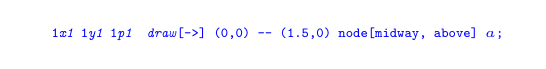
\begin{tikzpicture}
   		\draw[->] (0,0) -- (1.5,0) node[midway, above] {$a$};
   	\end{tikzpicture}\hspace{.7em} δηλώνει πολλαπλασιασμό με τον αριθμό \( a \)
   	\item 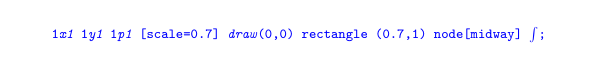
\begin{tikzpicture}[scale=0.7]
   		\draw (0,0) rectangle (0.7,1) node[midway] {$\int$};
   	\end{tikzpicture}\hspace{.7em} σημαίνει ολοκλήρωση
   	\end{itemize}
   \end{infobox}


   \begin{align}
   	\int a(x+r) \dif t &= r \xRightarrow{\sfrac{\dif}{\dif t} } \od{r}{t} = ax+ar
   	 \label{eq:ex21}
   	\\ r+b\int r\dif t &= y \implies \od{r}{t} + br = \od{y}{t} \label{eq:ex22}
   	\end{align}
   	\begin{align*}
   	\eqref{eq:ex21} - \eqref{eq:ex22} \implies r(a+b) &= \od{y}{t} - ax \\
   	r &= \frac{1}{a+b} \left(\od{y}{t} - ax\right) \\
   	\frac{\od[2]{y}{t}-a\od{x}{t}}{a+b} + \frac{-a}{a+b} \left(
   	\od{y}{t}-ax
   	\right) = ax \\
   	\od[2]{y}{t} - a\od{y}{t} &= a\od{x}{t} + abx
   	\implies \\ \implies s^2Y(s) - asY(s) &= asX(s) + abX(s) \\
   	\implies \frac{Y(s)}{X(s)} &= H(s) = \frac{a(s+b)}{s(s-a)}
   \end{align*}

   Αν \( \Re\left\lbrace a \right\rbrace < 0 \), τότε
   \( \displaystyle H(\omega ) = \frac{a(j\omega +b)}{j\omega (j\omega -a)} \)

    \begin{infobox}{Ένα διάγραμμα όπως τα παρακάτω μπορεί να περιέχει:}
    	\subparagraph{Τελεστή άθροισης}
    	\( y(t) = x(t) + v(t) \pm w(t) \)

	    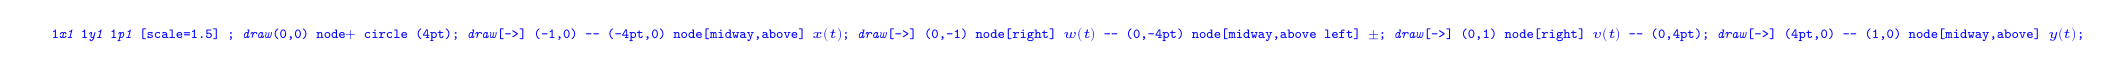
\begin{tikzpicture}[scale=1.5]
	    \def\cr{4pt};

	    \draw (0,0) node{$+$} circle (\cr);

	    \draw[->] (-1,0) -- (-\cr,0) node[midway,above] {$x(t)$};
	    \draw[->] (0,-1) node[right] {$w(t)$} -- (0,-\cr) node[midway,above left] {$\pm$};
	    \draw[->] (0,1) node[right] {$v(t)$} -- (0,\cr);
	    \draw[->] (\cr,0) -- (1,0) node[midway,above] {$y(t)$};
	    \end{tikzpicture}

	    \subparagraph{Γινόμενο συνάρτησης με αριθμό}
	    \( y(t) = ax(t) \)

	    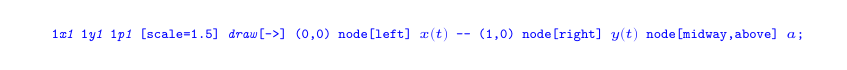
\begin{tikzpicture}[scale=1.5]
	    	\draw[->] (0,0) node[left] {$x(t)$} --
	    	(1,0) node[right] {$y(t)$} node[midway,above] {$a$};
	    \end{tikzpicture}

	    \subparagraph{Συνέλιξη} \hspace{0pt}

	    \begin{tikzpicture}[scale=1.2]
	    	\draw[->] (0,0) -- (1,0) node[above,midway] {$x(t)$} ;
	    	\draw (1,0.25) rectangle (2.3,-0.25) node[midway] {$h_1(t)$};
	    	\draw[->] (2.3,0) -- (3.3,0) node[above,midway] {$y(t)$}
	    	node[xshift=5mm,right] {$y(t) = h_1(t) * x(t)$};

	    	\begin{scope}[yshift=-1cm]
	    	\draw[->] (0,0) -- (1,0) node[above,midway] {$x(t)$} ;
	    	\draw (1,0.25) rectangle (2.3,-0.25) node[midway] {$H_1(s)$};
	    	\draw[->] (2.3,0) -- (3.3,0) node[above,midway] {$y(t)$}
	    	node[xshift=5mm,right] {$Y(s) = H_1(s) X(s)$};
	    	\end{scope}

	    	\draw[thick,decorate,decoration={brace,amplitude=10pt}]
	    	(3.4,0.5) -- (3.4,-1.5);

	    	\draw (8,-1) node
	    	{$\mathsmaller{\mathsmaller{
	    				H_1(s) = \mathscr L \left\lbrace h_1(t)\right\rbrace}}$};
	    \end{tikzpicture}

	    \subparagraph{Συνδυασμός (σε σειρά)}
	    \( y(t) = h_2(t) * v(t) = h_2(t) * \left(x(t)*h_1(t)\right) =
	    \left[h_1(t) * h_2(t)\right] * x(t)
	     \)

	    \begin{tikzpicture}[scale=1.3]
	    	\draw[->] (0,0) -- (1,0) node[above,midway] {$x(t)$} ;
	    	\draw (1,0.25) rectangle (2.3,-0.25) node[midway] {$h_1(t)$};
	    	\draw[->] (2.3,0) -- (3.3,0) node[midway] (V) {};
	    	\draw (3.3,0.25) rectangle (4.6,-0.25) node[midway] {$h_2(t)$};
	    	\draw[->] (4.6,0) -- (5.6,0) node[right] {$y(t)$};

	    	\filldraw[blue!50!green] (V) circle (1pt) node[above] {$v(t)$};

	    	\draw ({(1+2.3)/2},-0.7)
	    	node {$\mathlarger{\mathlarger{\mathlarger{\mathlarger{\Updownarrow}}}}$};

	    	\begin{scope}[yshift=-1.4cm]
	    	\draw[->] (0,0) -- (1,0) node[above,midway] {$x(t)$} ;
	    	\draw (1,0.25) rectangle (2.3,-0.25) node[midway] {$\mathsmaller{h_1(t)*h_2(t)}$};
	    	\draw[->] (2.3,0) -- (3.3,0) node[above,midway] {$y(t)$};
	    	\end{scope}
	    \end{tikzpicture}

	    ή

	    \begin{tikzpicture}[scale=1.3]
	    	\draw[->] (0,0) -- (1,0) node[above,midway] {$x(t)$} ;
	    	\draw (1,0.25) rectangle (2.3,-0.25) node[midway] {$H_1(s)$};
	    	\draw[->] (2.3,0) -- (3.3,0);
	    	\draw (3.3,0.25) rectangle (4.6,-0.25) node[midway] {$H_2(s)$};
	    	\draw[->] (4.6,0) -- (5.6,0) node[right] {$y(t)$};

	    	\draw ({(1+2.3)/2},-0.7)
	    	node {$\mathlarger{\mathlarger{\mathlarger{\mathlarger{\Updownarrow}}}}$};

	    	\begin{scope}[yshift=-1.4cm]
	    	\draw[->] (0,0) -- (1,0) node[above,midway] {$x(t)$} ;
	    	\draw (1,0.25) rectangle (2.3,-0.25) node[midway] {$\mathsmaller{H_1(s)H_2(s)}$};
	    	\draw[->] (2.3,0) -- (3.3,0) node[above,midway] {$y(t)$};
	    	\end{scope}
	    \end{tikzpicture}


	    \subparagraph{Συνδυασμό (παράλληλα)} \hspace{0pt}

	    \begin{tikzpicture}[scale=1.3]
	    \def\cr{4pt};

	    \draw[->] (-1,0) -- (0,0) node[above,midway] {$x(t)$} ;
	    \draw[->] (0,0) -- (0,0.75) -- ++(1,0);
	    \draw (1,1) rectangle ++(1.3,-0.5) node[midway] {$h_1(t)$};
	    \draw[->] (2.3,0.75) -- ++(1,0) -- (3.3,\cr);
	    \draw[->] (0,0) -- (0,-0.75) -- ++(1,0);
	    \draw (1,-1) rectangle ++(1.3,0.5) node[midway] {$h_2(t)$};
	    \draw[->] (2.3,-0.75) -- ++(1,0) -- (3.3,-\cr);

	    \draw (3.3,0) node {$+$} circle (\cr);
	    \draw[->] (3.3cm+\cr,0) -- ++(1,0) node[above,midway] {$y(t)$};

	    \draw ({(1+2.3)/2},-1.4)
	    node {$\mathlarger{\mathlarger{\mathlarger{\mathlarger{\Updownarrow}}}}$};

	    \begin{scope}[yshift=-2.1cm]
	    \draw[->] (0,0) -- (1,0) node[above,midway] {$x(t)$} ;
	    \draw (1,0.25) rectangle (2.3,-0.25) node[midway] {$\mathsmaller{h_1(t)+h_2(t)}$};
	    \draw[->] (2.3,0) -- (3.3,0) node[above,midway] {$y(t)$};
	    \end{scope}
	    \end{tikzpicture}

	    \subparagraph{Τελεστές} \hspace{0pt}

	    
\begin{tikzpicture}[scale=1,baseline]
	    \draw[->] (0,0) -- (1,0) node[above,pos=.4] {$x(t)$};
	    \draw (1,0.35) rectangle (1.4,-0.35) node[midway] {$\int$};
	    \draw[->] (1.4,0) -- ++(1,0) node[above,pos=.5] {$y(t)$};
	    \end{tikzpicture}
	    \( y(t) = \int_{-\infty}^{t} x(\tau) \dif\tau \)

	    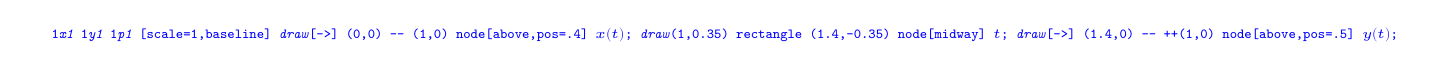
\begin{tikzpicture}[scale=1,baseline]
	    \draw[->] (0,0) -- (1,0) node[above,pos=.4] {$x(t)$};
	    \draw (1,0.35) rectangle (1.4,-0.35) node[midway] {$\od{}{t}$};
	    \draw[->] (1.4,0) -- ++(1,0) node[above,pos=.5] {$y(t)$};
	    \end{tikzpicture}
	    \( y(t) = \od{x}{t} \)
    \end{infobox}

    \newpage

    \paragraph{Άσκηση}
    Να βρεθεί το ισοδύναμο του block diagram:

    \begin{tikzpicture}
    \def\cr{7pt};
    \draw[->] (0,0) -- (1cm-\cr,0)
    node[midway,above] {$x(t)$} node[midway,below] {$X(s)$};
    \draw (1,0) node {$+$} circle (\cr);
    \draw[->] (1cm+\cr,0) -- (2.1,0) node [midway,below] (A) {};
    \draw (2.1,0.25) rectangle ++(1.5,-0.5) node[midway] {$H_1(s)$};

    \draw[->,green!50!black] (A) -- ++(0,1) node[above] {$\Xi(s)$};
    \draw[->] (3.6,0) -- (5,0) node[right] {$y(t)$} node[below right,yshift=-2mm] {$Y(s)$};

    \draw[->] (4.6,0) -- ++(0,-1) -- (3.6,-1);
    \draw (2.1,0.25-1) rectangle ++(1.5,-0.5) node[midway] {$H_2(s)$};
    \draw[->] (2.1,-1) -- (1,-1) -- (1,-\cr);

    \draw (2.85,-2)
    node {$\mathlarger{\mathlarger{\mathlarger{\mathlarger{\Updownarrow}}}}$};

    \begin{scope}[yshift=-3cm]
    \draw[->] (1,0) -- (2.1,0) node[midway,above] {$x(t)$};
    \draw (2.1,0.25) rectangle ++(1.5,-0.5) node[midway] {$H(s)$};
    \draw[->] (3.6,0) -- (5,0) node[midway,above] {$y(t)$};
    \end{scope}
    \end{tikzpicture}
    \begin{align*}
    	Y(s) &= H_1(s) \cdot \Xi(s) \\
    	&= H_1(s) \cdot \left[ X(s) + Y(s) \right] \implies \\
    	Y(s) &= H_1(s) \left[ X(s)+H_2(s)Y(s) \right] \implies \\
    	Y(s) \left[1-H_1(s)H_2(s)\right] &= H_1(s)X(s) \\[.3em]
    	Y(s) &= H(s) X(s) \\
    	H(s) &= \frac{Y(s)}{X(s)} = \frac{H_1(s)}{1-H_1(s)H_2(s)}
    \end{align*}

    \paragraph{Άσκηση}
    \hspace{0pt}

    
\begin{tikzpicture}[scale=1.2]
    \def\cr{7pt};
    \draw[->] (-0.5,0) -- (1cm-\cr,0) node[midway,above] {$x(t)$};
    \draw (1,0) node {$+$} circle (\cr);
    \draw[->] (1cm+\cr,0) -- (2.1,0) node [midway,below] (A) {};
    \draw (2.1,0.3) rectangle ++(3,-0.6) node[midway]
    {$\ddot o + 5\dot o +6o = \dot\imath + \imath$};

    \draw[->] (5.1,0) -- (6.5,0) node[right] {$y(t)$}
    node[below right,yshift=-2mm] {};

    \draw[->] (6,0) -- ++(0,-1) -- (4.55,-1);
    \draw (2.55,0.25-1) rectangle ++(2,-0.5) node[midway] {$\dot o + o = \imath$};
    \draw[->] (2.55,-1) -- (1,-1) -- (1,-\cr);

    \draw (3.6,0.25) node[above,green]
    {$\mathsmaller{H_1: \ s^2O(s)+5sO(s)+6O(s)=sI(s)+I(s)}$};
    \draw (3.6,-1.25) node[below,green]
    {$\mathsmaller{H_2: \ sO(s)+O(s)=I(s)}$};

    \draw[dashed,gray] (0.6, 0.8) rectangle (6.3,-1.8);

    \draw (2.85,-2)
    node {$\mathlarger{\mathlarger{\mathlarger{\mathlarger{\Updownarrow}}}}$};
    \end{tikzpicture}

    \begin{align*}
    	H_1(s) &= \frac{O(s)}{I(s)} = \frac{s+1}{s^2+5s+6} = \frac{s+1}{(s+3)(s+2)} \\
    	H_2(s) &= \frac{O(s)}{I(s)} = \frac{1}{s+1}
    	\intertext{\( H_1,H_2 \) ευσταθή,
    		αφού οι πόλοι τους βρίσκονται στο αριστερό ημιεπίπεδο}
    	Y(s) &= H_1(s) \cdot \left[ X(s) - H_2(s)Y(s) \right] \implies
    	\frac{Y(s)}{X(s)} = H(s) = \frac{H_1(s)}{1+H_1(s)H_2(s)}
    \end{align*}


    \paragraph{Άσκηση} \hspace{0pt}

    
\begin{tikzpicture}
    \draw[->] (0,-2) -- (0,2) node[above] {$i\omega$};
    \draw[->] (-2,0) -- (2,0) node[below] {$\sigma$};

    \draw (1,1) node[above right] {$s$-plane};

    \draw (-0.75,0) node[cross=3pt,thick,red] {} node[below,yshift=-1mm] {$-0.5$};
    \draw (-1.5,0) node[cross=3pt,thick,red] {} node[below,yshift=-1mm] {$-1$};

    \draw plot [smooth]
    coordinates {(-1.5,-0.7) ({(-0.75-1.5)/2},-1.1) (-0.75,-0.7)};
    \draw[->] ({(-0.75-1.5)/2},-1.1) -- ++(0,-0.5) node[below,rectangle,align=center]
    {απλοί πόλοι,\\δεν έχει μηδενικά};
    \end{tikzpicture}

    Αν η είσοδος \( x(t) = \mathrm u(t) \), βρίσκω μετά από "πολλά χρόνια" ότι \( y(t)=1
    \implies \lim_{t\to \infty} y(t) = 1
    \). Να βρεθεί ολόκληρη η \( y(t) \).

    \begin{align*}
   	    H(s) &= \frac{k}{(s+1)\left(s+\sfrac{1}{2} \right)} \\
   	    Y(s) &= H(s)X(s) = \frac{k}{(s+1)\left(s+\sfrac{1}{2} \right)}\frac{1}{s} \\
   	    \text{Όμως } \lim_{t\to \infty} y(t) &= \lim_{s \to 0} sY(s) \\
   	    1 &= \lim_{s\to 0}
   	    \left[\frac{k}{(s+1)\left(s+\sfrac{1}{2} \right)}\frac{1}{s}s\right] = 2k \implies
   	    \boxed{k = \sfrac{1}{2} } \\
   	    \text{Άρα }
   	    Y(s) &= \frac{\sfrac{1}{2} }{s(s+1)\left(s+\sfrac{1}{2} \right)}
   	    = \frac{1}{s} + \frac{1}{s+1} + \frac{-2}{s+\sfrac{1}{2} } \\
   	    y(t) &= \left[ 1+e^{-t} -2e^{\sfrac{-t}{2} } \right]\mathrm{u}(t)
    \end{align*}

    \paragraph{Άσκηση}
    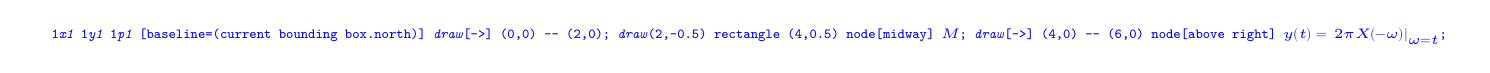
\begin{tikzpicture}[baseline=(current bounding box.north)]
    	\draw[->] (0,0) -- (2,0);
    	\draw (2,-0.5) rectangle (4,0.5) node[midway] {$M$};
    	\draw[->] (4,0) -- (6,0) node[above right]
    	{$y(t) = \left. 2\pi X(-\omega )\right|_{\omega = t}$};
    \end{tikzpicture}

    όπου \( X(\omega ) = \mathrm{FT}\left\lbrace x(t) \right\rbrace \)

    
\begin{tikzpicture}[scale=1.2]
    \draw[->,yshift=-0.5mm] (0,0) -- (1,0) node[midway,above] {$x(t)$};
    \draw (1,0.25) rectangle (2,-0.25) node[midway] {$M$};
    \draw[->] (2,0) -- (3,0) node[blue,midway,below] {$\mathsmaller{(1)}$};
    \draw (3,0.25) rectangle (4,-0.25) node[midway] {$M$};
    \draw[->] (4,0) -- (5,0) node[blue,midway,below] {$\mathsmaller{(2)}$};
    \draw (5,0.25) rectangle (6,-0.25) node[midway] {$M$};
    \draw[->] (6,0) -- (7,0) node[blue,midway,below] {$\mathsmaller{(3)}$};
    \draw (7.2,0) node {$\times$} circle (0.2);
    \draw[->] (7.4,0) -- (8,0) node[right] {$w(t)$};

    \draw[<-] (7.2,-0.2) -- ++(0,-0.5) node[below] {$\left(\frac{1}{2\pi}\right)^4$};
    \end{tikzpicture}

    Για να υπάρχει συνάρτηση μεταφοράς του \( M \), πρέπει να είναι γραμμικό \& αμετάβλητο:

    \begin{align*}
    	x(t) &\to 2\pi X(-t) \\
    	y(t) &\to 2\pi Y(-t) \\
    	ax+\beta y\ (t) &\to a2\pi X(-t) + \beta 2\pi Y(-t) \text{ good} \\[.3em]
    	x(t) &\to \left. 2\pi X(-\omega ) \right|_{\omega = t} \\
    	y(t) &\to 2\pi e^{-j\tau} X(-\tau)
    \end{align*}

    Έχω:
    \begin{align*}
    	y_1(t) &= \left. 2\pi X(-\omega )\right|_{\omega =t}
    	= \left.2\pi \int_{-\infty}^{\infty} x(\tau_1) e^{-j\tau_1(-\omega )}\dif\tau_1
    	\right|_{\omega =t}
    	=2\pi \int_{-\infty}^{\infty} x(\tau_1) e^{j\tau_1 t}\dif\tau_1 \\
    	y_2(t) &= \left. 2\pi Y_1(-\omega )\right|_{\omega =t}
    	= \left.2\pi \int_{-\infty}^{\infty} y_1(\tau_2) e^{-j\tau_2(-\omega )}\dif\tau_2
    	\right|_{\omega =t}
    	\\ &=\left. 2\pi \int_{-\infty}^{\infty} 2\pi
    	\int_{-\infty}^{\infty} x(\tau_1) e^{j\tau_1\tau_2}\dif\tau_1 e^{-j\tau_2(-\omega)}
    	\dif\tau_2\right|_{\omega = t}
    	\\ &= (2\pi)^2 \int_{-\infty}^{\infty} x(\tau_1) \int_{-\infty}^{\infty}
    	e^{j\tau_2(\tau_1+t)}\dif\tau_2\dif\tau_1
    	\\ &= (2\pi)^2 \int_{-\infty}^{\infty} x(\tau_1)2\pi \delta(\tau_1+t)\dif\tau_1
    	= (2\pi)^3 \int_{-\infty}^{\infty} x(\tau_1)\delta(\tau_1+t)\dif\tau_1 =
    	(2\pi)^3 x(-t) \\
    	Y_2(\omega) &= (2\pi)^3 X(-\omega) \\
    	y_3(t) &= \left. 2\pi Y_2(-\omega ) \right|_{\omega =t}
    	= \left. (2\pi)^3 X(\omega ) \right|_{\omega = t} \\ &= (2\pi)^4 X(t)
    \end{align*}

    \begin{attnbox}{}
    	Στις εξετάσεις θα κουβαλήσουμε ένα δικό μας μαθηματικό τυπολόγιο
    	(π.χ. Schaum's Tables \& Formulas)
    \end{attnbox}
\end{document}
